\chapter{Discovering the Control-Flow Perspective}
\label{chap:project-mining2}

{\bfseries \Large Authors: \medskip}

Saimir Bala,
Paul Kneringer, and
Jan Mendling \hfill

\bigskip

{\noindent\bfseries \Large Published in: \medskip}

Proceedings of the Forum at Practice of Enterprise Modeling 2020 co-located
with the 13th {IFIP} {WG} 8.1 Working Conference on the Practice of
Enterprise Modeling (PoEM 2020), Riga, Latvia, November 25-27, 2020

\bigskip

{\noindent\bfseries \Large Abstract: \medskip}


Software development processes are complex to monitor as they involve the coordination of many resources working with different tools.
This makes it hard to apply mining techniques for monitoring the process. 
A key challenge for using traces of tools such as version control systems (VCS) is to find meaningful abstractions in order to identify the work that was actually done. 
In this paper, we use data from VCS to analyze the actual progress of software-development processes. We develop a technique that is able to mine the activity types of which the development processes consists. 
We implement our technique as a prototype in Java and evaluate its outputs in terms of effectiveness.
In this way, we are able to graphically uncover new behavioural patterns in real-world data from existing open-source GitHub repositories.

\pagebreak


%	
Software development processes are complex to monitor as they involve the coordination of many resources working with different tools.
This makes it hard to apply mining techniques for monitoring the process. 
A key challenge for using traces of tools such as version control systems (VCS) is to find meaningful abstractions in order to identify the work that was actually done. 
In this paper, we use data from VCS to analyze the actual progress of software-development processes. We develop a technique that is able to mine the activity types of which the development processes consists. 
We implement our technique as a prototype in Java and evaluate its outputs in terms of effectiveness.
In this way, we are able to graphically uncover new behavioural patterns in real-world data from existing open-source GitHub repositories.



%%
\section{Introduction}


Software development processes involve the coordination of multiple resources working on different parts of the software at the same time. As these resources focus on specific parts of the overall development process, it is difficult to obtain  transparency of the current status of the project. At the same time, monitoring such process is required in order to avoid risks of running out of time, budget or not meeting established quality objectives.

These type of processes have been referred to as \emph{project-oriented} business processes or simply as \emph{projects}. Monitoring a project is complex because there is hardly any central control of the work progress. 
% However, there is a myriad of trace data from different systems that is generated every day. One fundamental system in modern software projects are \glspl{vcs}. 
One type of system that is extensively used in software development are \glspl{vcs}.
They are used to keep track of the changes of the different files that constitute a project. Trace data generated by \gls{vcs} is a starting point for mining these type of processes. However, only a few approaches~\cite{DBLP:conf/bpm/BalaCMRP,DBLP:conf/bpm/JookenCJ19}  focus on analyzing the status of software development from these fine-grained \gls{vcs} traces. Thus, there is a need to fill in this gap with further techniques that allow to identify additional aspects of the development process, such as the actual activities done by developers. 

% On the other hand, there is a myriad of trace data from different systems that is generated every day. One fundamental system in modern software projects are \glspl{vcs}. These systems are used to keep track of the changes of the different files that constitute a project. Trace data generated by these systems is a starting point for mining software development processes. So far, only a few approaches exist (such as~\cite{DBLP:conf/bpm/BalaCMRP,DBLP:conf/bpm/JookenCJ19}) that help analyzing the status of software development. Support for understanding which types of work where conducted is missing.

In this paper, we provide a technique for capturing the progress of a project in such a way that it becomes clear what work activity is being done over time. We define fundamental concepts for representing these processes, upon which we develop a novel analysis technique. Our prototypical implementation of this technique is able to represent the status of the development process as well as the activity that is being done. 
%Kate: [2] was not explained so it is not clear the extension. This works advances the state-of-the art on project mining by extending the information offered by the technique developed by~\cite{DBLP:conf/bpm/BalaCMRP}.

The rest of the paper is organized as follows. \Cref{sec:background} details the problem, positions our contribution against existing literature, and defines the requirements for the design of the artifact that solves the stated problem. 
\Cref{sec:approach} defines preliminary concepts and presents the approach to mine the activities. %Kate: you describes the implementation in the section before 
\Cref{sec:results} describes the implementation of the artifact and shows its application to real-world projects. 
% \Cref{sec:discussion} highlights the implications of our results for project managers. 
\Cref{sec:conclusion} concludes the paper.
%%
%
%\section{Background}
%\label{sec:background}

% This section provides the problem description, derives the requirements of the solution and positions our work against the current state-of-the-art.

\section{The Problem of Control-Flow Discovery}
\label{sec:problem}

Control-flow discovery consists of finding out a model of that displays ordering relations between activities of a process. This is useful when it comes to monitoring software engineering projects. Given software repository trace data, the goal is to automatically infer the type of work that is reflected by the change of the artifacts. 
% These type of processes have also been referred to as \glspl{pobp}~\cite{DBLP:conf/bpm/BalaCMRP}. In this paper we simply refer to them as \emph{projects}. 
%These projects present the following characteristics. First, they are hardly repetitive. That is, while best practices learned from one project or can be reused, it is never the case that the project is rerun exactly in the same way. Second, they are worked on collaboratively by many participants who regularly document their progress in a semi-structured way. %They want to document progress is typically through semi-structured artifacts such as textual data or tables. 
%Third, the work is performed under clear constraints in terms of time, budget and quality. Fourth, the workflow does not follow an imperative process model and is not managed by a process engine. Fifth, despite the aforementioned limitations, project managers require transparency of the process in terms of being able to distinguish what kind of work activities where done when and by which resource. 
In the following, we consider the terms ``type-of-work'' and ``activity'' as synonyms.

% \todo[inline]{See the link I sent. Use Sebok and describe its major categories of ISD tasks. cite~\cite{bourque2014guide}.}

%Kate: is the following necessary? Do you need to talk about RUP?
% According to the \gls{swebok}~\cite{bourque2014guide} guide software engineering consists of the following main activities: 
% \begin{inparaenum}[\itshape i)]
% \item software requirements;
% \item software design;
% \item software construction;
% \item software testing; and
% \item software maintenance.
% \end{inparaenum} These activities are mostly seen as areas of software engineering. They contain sub-activities which vary based on the adopted methodology. For instance, agile software development might focus on the necessary activities required for releasing a new version of a software, such as development and testing. On the other hand, a more classic methodology such as waterfall, might allocate more time to the analyses and definition of the requirements. Although different methodologies may exist, software development work can be broken down into specific types of work that need to be performed at specific times as defined by the \gls{rup} model~\cite{kruchten2004rational}. 

%Project managers need tools that help them understand where the project is currently standing and how they have performed in retrospect. Being able to see what work was done and when opens up possibilities to understand inefficiencies about how the process was conducted. Moreover, managers need to access information in a timely manner. Therefore, a representation of progress over time is important. Theoretical models of the development process, such as the \gls{rup}, are useful for planning software projects but they fall short when it comes to monitoring.
%
%Fortunately, software development projects store rich trace data. Participants (e.g., resources, users) use many tools for different purposes. A common tools is used in any professional software engineering project are \glspl{vcs}. These systems allow users to collaboratively work on the same project. They manage the different versions of files created by users at any point in time. As well, they keep track of all the changes done by resources at all times. These kind of systems represent a starting point for analyzing projects. As software projects may contain hundreds of thousands files, it becomes prohibitive to manually check what work was done in the project. This calls for automatic analyses and reporting. 
% to understand how the work is distributed among project members. 

% Let us show an example of how a version control is used to develop a software. 

%\begin{table}[bt]
\caption{Excerpt from VCS log data for the referenced time period. \todo[inline]{This table was already used in the BPM2015 paper. Change it!}}
\label{tab:example}
\scriptsize
{\renewcommand{\arraystretch}{1.3}
\centering
%\fontfamily{phv}\fontseries{mc}\selectfont
\begin{tabular}{m{.8cm} m{1.5cm} m{3cm} p{5.8cm}}
\hline\noalign{\smallskip}
%\hline
\textbf{CID}	 & \textbf{Resource} & \textbf{Date} & \textbf{List of changes} \\
%\noalign{\smallskip}
\hline
%\noalign{\smallskip}
\hline
\noalign{\smallskip}
\multirow{2}{*}{1} & \multirow{2}{*}{Y} & \multirow{2}{*}{2014-11-12~11:57:46} & A /example \\
& & & A \slash example\slash SHAPE\slash\-ToyStation\-Example.docx \\ \hline %\hdashline

%\multirow{2}{*}{205} & \multirow{2}{*}{X} & \multirow{2}{*}{2014-11-14 16:26:23} & A /example/ToyStation.bpmn \\
%& & & A /example/ToyStation.png \\ \hline %\hdashline

\ldots & \ldots & \ldots & \ldots \\ \hline

\noalign{\smallskip}
\multirow{2}{*}{3} & \multirow{2}{*}{X} & \multirow{2}{*}{2014-11-14 16:34:07} & M /example/ToyStation.bpmn\\
& & & M /example/ToyStation.png \\ \hline %\hdashline

%\multirow{7}{*}{207} & \multirow{7}{*}{X} & \multirow{7}{*}{2014-11-27 14:18:59} & M /example/SHAPE-ToyStation-Example.docx \\
%& & & D /example/ToyStation.bpmn \\
%& & & M /example/ToyStation.png \\
%& & & A /example/ToyStation\_0Loop.bpmn \\
%& & & A /example/ToyStation\_1Loop.bpmn \\
%& & & A /example/ToyStation\_nLoop.bpmn \\
%& & & A/example/ToyStation\_old.bpmn\\ \hline

%\ldots & \ldots & \ldots & \ldots \\ \hline

\noalign{\smallskip}
4 & W & 2014-12-15 13:49:11 & D /example/Download \\ \hline %\hdashline

\noalign{\smallskip}
5 & W & 2015-01-08 16:06:41 & A /example/Download2\\ \hline %\hdashline

\noalign{\smallskip}
\multirow{2}{*}{6} & \multirow{2}{*}{X} & \multirow{2}{*}{2015-01-13 11:47:09} & M /example/ToyStation\_0Loop.bpmn\\
& & & M /example/ToyStation\_nLoop.bpmn \\ \hline %\hdashline

\noalign{\smallskip}
\multirow{2}{*}{7} & \multirow{2}{*}{Z} & \multirow{2}{*}{2015-01-16 16:50:29} & A /example/ToyStation\_0Loop.pdf\\
& & & A /example/ToyStation-feedbackZ.pdf\\ \hline %\hdashline
\end{tabular}\\ \hfill
}
\end{table}
%\todo{if we are short of space, this can be shortened. This text should not be more than something like a quarter of a page.}

\lstset{
  basicstyle={\normalsize\ttfamily}}
  
Typical \emph{activities} (i.e., type of work) traced by \glspl{vcs} fall under the categories \textsl{Code}, \textsl{Documentation}, \textsl{Test}, etc. Major \glspl{vcs} like Git and Subversion, do not provide direct support for understanding the activities executed by developers. However, these tools provide rich event logs which record all the changes made to any file. %\Cref{tab:example}
\Cref{lst:git-log} presents an excerpt of trace data from a publicly available GitHub repository. Specifically, the trace data shows information about two commits, which are activities performed by developers to save their work progress. These commits have a unique identifier and provide information about \begin{inparaenum}[\itshape i)]
\item the author (i.e., the human resource who issued the commit);
\item the date (i.e., a timestamp recording the instant when the commit was made);
\item a natural-language textual description filled in by the author; and
\item a list of files that were either modified (M), added (A) or deleted (D).
\end{inparaenum}

\lstset{frame=tb,
  aboveskip=3mm,
  belowskip=3mm,
  showstringspaces=false,
  columns=flexible,
  basicstyle={\scriptsize\ttfamily},
  numbers=none,
  xleftmargin=.05\textwidth,
  xrightmargin=.05\textwidth,
 % linewidth = 0.7\textwidth,
  numberstyle=\tiny\color{gray},
  keywordstyle=\color{blue},
  commentstyle=\color{dkgreen},
  stringstyle=\color{mauve},
  breaklines=true,
  breakatwhitespace=true,
  tabsize=3
}
\renewcommand{\thelstlisting}{\arabic{lstlisting}}

\begin{lstlisting}[caption={Excerpt from VCS log data from git},label={lst:git-log}]
commit b0346a47df142394da820e1e5d0f7e31b41a70d3
Author: s41m1r 
Date:   Wed Feb 4 13:05:14 2015 +0100

    Deleted TODOs

D	MiningSVN/TODOs
M	MiningSVN/src/reader/GITLogReader.java

commit 30c5e536e88501295aa3f226645953c69e8f3947
Author: s41m1r 
Date:   Wed Feb 4 15:31:05 2015 +0100

    Works with GIT (hopefully)

M	MiningSVN/src/model/git/GITLogEntry.java
M	MiningSVN/src/reader/GITLogReader.java
M	MiningSVN/src/reader/LogReader.java
M	MiningSVN/src/test/TestReadDate.java
A	MiningSVN/src/test/TestReadGIT.java
M	MiningSVN/src/test/TestReadSVNLog.java
\end{lstlisting}





% Real-life software projects may account for hundreds of thousands of commits. Thus, the amount of data contained in these event logs is infeasibly large to be analyzed manually. Therefore, the type of work activities should be automatically inferred by these events. 
As real-life event logs may contain a large amount of commits, it is imperative to use automatic tools to discover the activities. 
While it is possible to take into account the commit messages and apply \gls{nlp} techniques to classify the various changes~\cite{DBLP:conf/edoc/AgrawalATBRT16}, \Cref{lst:git-log} suggests that there are no guarantees that the textual descriptions are informative about the activity. For this reason, this work focuses on the type of file
that was modified rather than relying of the commit comments. 

% \subsection{Requirements}
Therefore, the problem is how to exploit low-level trace data for extracting project knowledge that is informative to the manager. We translate this problem into the following requirements.
% which must be fulfilled by an artifact to be useful to a project manager.

\noindent
\begin{inparadesc}
\item[RQ1. (Processing of \gls{vcs} event logs).] The prototype must extract valuable information from\gls{vcs} data. \\
\item[RQ2. (Identification of the activities).] The prototype shall classify what activity is done and when.\\
\item[RQ3. (Computation of KPIs).] The prototype shall provide \glspl{kpi} that are understandable by project managers.\\
\item[RQ4. (Visualization of project status).] The prototype shall provide a high level overview of the project.
\end{inparadesc}



\section{Related work}
\label{subsec:requirements}

Literature related to the aforementioned requirements can be classified into two main groups: \begin{inparaenum}[\itshape (i)]
\item software engineering; and 
\item business process management.
\end{inparaenum} 
% \Cref{tab:literature} gives an overview of this categorization against the identified requirements. 

% % Please add the following required packages to your document preamble:
% \usepackage{booktabs}
% \usepackage{multirow}
\begin{table}[htbp]
\caption{Positioning this contribution against existing literature. Symbols semantics: requirement \cmark addressed; $\sim$ partially addressed; \xmark~not addressed}
\label{tab:literature}
\begin{tabular}{@{}llllll@{}}
\toprule
\textbf{\begin{tabular}[c]{@{}l@{}}Research \\ area\end{tabular}} &
  \textbf{Approaches} &
  \textbf{\begin{tabular}[c]{@{}l@{}}Process \\ VCS event \\ logs\end{tabular}} &
  \textbf{\begin{tabular}[c]{@{}l@{}}Visualize \\ project \\ status\end{tabular}} &
  \textbf{\begin{tabular}[c]{@{}l@{}}Visualize \\ type of \\ work\end{tabular}} &
  \textbf{\begin{tabular}[c]{@{}l@{}}Compute \\ KPIs\end{tabular}} \\ \midrule
\multirow{4}{*}{MSR} & Zimmermann~\cite{DBLP:journals/tse/ZimmermannWDZ05}      & \cmark & {{$\mathbb \sim$}} & \cmark & {{$\mathbb \sim$}} \\
& Zaidman et al.~\cite{DBLP:conf/icst/ZaidmanRDD08}        & \cmark & {{$\mathbb \sim$}} & \xmark & \xmark \\
                     & Oliva et al.~\cite{DBLP:conf/iwpse/OlivaSGS11}           & \cmark & \xmark & \xmark & \xmark \\
                     & Vasilescu et al.~\cite{DBLP:journals/ese/VasilescuSGM14} & \cmark & {{$\mathbb \sim$}} & \xmark & \cmark \\ 
                     & Rodriguez et al.~\cite{DBLP:conf/msr/RodriguezTK18}      & \cmark & {{$\mathbb \sim$}} & \cmark & {{$\mathbb \sim$}} \\
                     & Joonbakhsh \& Sami~\cite{DBLP:conf/msr/JoonbakhshS18}      & \cmark & {{$\mathbb \sim$}} & \cmark & {{$\mathbb \sim$}} \\
                     \midrule
\multirow{7}{*}{\begin{tabular}[c]{@{}l@{}}Process /\\ Project Mining\end{tabular}} &
  Bala et al.~\cite{DBLP:conf/bpm/BalaCMRP} &
  \cmark &
  \cmark &
  \xmark &
  \cmark \\
                     & Kindler et al.~\cite{DBLP:conf/se/KindlerRS06}           & \cmark & \xmark & {{$\mathbb \sim$}} & \xmark \\
                     & Poncin et al.~\cite{DBLP:conf/csmr/PoncinSB11}           & \cmark & {{$\mathbb \sim$}} & {{$\mathbb \sim$}} & \xmark \\
                     & Bentallah et al.~\cite{DBLP:conf/caise/BeheshtiBN13}     & \cmark & {{$\mathbb \sim$}} & {{$\mathbb \sim$}} & \xmark \\
                     & Marques et al.~\cite{DBLP:conf/wecwis/MarquesSF18}       & {{\xmark}} & {{$\mathbb \sim$}} & {{$\mathbb \sim$}} & {{$\mathbb \sim$}} \\
                     & Jooken et al.~\cite{DBLP:conf/bpm/JookenCJ19}            & \cmark & {{$\mathbb \sim$}} & {{$\mathbb \sim$}} & {{$\mathbb \sim$}} \\
                    %  & ActiVCS                                                  & \cmark & \cmark & \cmark & \cmark \\ 
                    \bottomrule
\end{tabular}
\end{table}



% In the software engineering area there is a dedicated conference aimed at working on this topic, namely \gls{msr}. 
Contributions in \textit{(i)} focus on event data generated by systems like \gls{vcs}, issue tracking, bug tracking, mail archives, etc. They mainly aim at either finding correlations between activities performed by resources and the artifacts in the repositories~\cite{DBLP:conf/iwpse/OlivaSGS11} or at analyzing the evolution of changes over time~\cite{DBLP:journals/tse/ZimmermannWDZ05}. These works typically provide powerful techniques that help with processing events~\cite{DBLP:conf/msr/0001W04} from software data and further abstracting them into coarse-grained activities~\cite{DBLP:conf/iwpse/OlivaSGS11,DBLP:conf/icst/ZaidmanRDD08,DBLP:conf/msr/RodriguezTK18} and 
 understanding type of work (i.e., activites) and \glspl{kpi}~\cite{DBLP:journals/ese/VasilescuSGM14,DBLP:conf/msr/JoonbakhshS18}.
While these works are fundamental in dealing with software repositories, they are typically process unaware. Therefore, do not provide a process representation.

Contributions in \textit{(ii)} fall under the \emph{process mining} umbrella. 
% Process mining helps discovering processes from log data. 
% However, all process mining techniques have specific requirements on the format about these event logs. That is, these techniques cannot be readily applied to data from software development~\cite{DBLP:conf/er/TsourySR18}. 
Typical approaches focus on transforming software development data in process-mining compatible event-logs~\cite{DBLP:conf/se/KindlerRS06,DBLP:conf/csmr/PoncinSB11}, by making assumptions on what to consider as a case identifier. Other works focus on enabling process analytics on top of fine-grained events from evolving artifacts~\cite{DBLP:conf/caise/BeheshtiBN13}. Finally, there are process-aware works that deal with software repositories. In particular, the work from~\cite{DBLP:conf/wecwis/MarquesSF18} analyses bug resolution processes and the work from~\cite{DBLP:conf/bpm/JookenCJ19} uses \gls{vcs} data to analyse teams. Most of the techniques in the process mining area have specific requirements about their input (i.e., an event log with defined case, activity, and timestamp attributes). These works cannot be readily applied to data from software development~\cite{DBLP:conf/er/TsourySR18}. 
In this paper, we focus on automatic identification of the activities based on file types as described in~\cite{DBLP:journals/ese/VasilescuSGM14}. Moreover, this work is process aware and presents the data from a perspective which is more targetted towards project managers.

% \textbf{RQ:} How can we make use of project trace data to gather insights about the software development process that are informative to managers?

% \cite{DBLP:conf/msr/RodriguezTK18} study IDE data
% \cite{DBLP:conf/msr/JoonbakhshS18} use IDE data to mine the Personal Software Process of developers. The result is similar to the Gantt chart by Bala et al., but shows only the amount of work for each developer. It does not provide any clue on the "type" of work the developer carried out. The user should know apriori what information is contained in the log (e.g., debugging logs --> debug activity), otherwise everything is "activity", mainly related to coding. 


%%
\section{Technique for discovering activities}
\label{sec:approach}

% In this section we illustrate the steps of the our technique for gathering insights on the software project (i.e., \gls{pobp}). Further, we discuss the design principles implemented by our prototype. 

% \subsection{Application scenario}

% Let us exemplify how our technique should help the project manager through the following four-step scenario.  
% First, using a \gls{gui}, a project manager should be able to analyze the project (i.e., explicitly see what activities are being done and when). She might observe a spike in a specific activity, for instance development. She notices that this is an unusual observation and she reports it for further investigation. This behaviour involves an exploration of the domain data in order to find interesting patterns. 
% Second, the manager describes this spike by using the information about the activity in which it occurred (e.g., in development and in testing), the time period (i.e., day, week, or month), the files and the resources involved. This description is needed in order to make the observation explicit and define it for further analysis.  
% Third, the manager crosses different observations on the data. She finds out that in the day before there were no changes by the resources in charge of that specific activity. She also observes that other resources who should not work on files affected by the spike, have actually made changes to those files. After cross-checking the resource occupancy with the day before, she finds out that actually resources were assigned bigger tasks which were not possible to be solved in the same day. That is why there was relatively little amount of work in the previous day and a sudden spike in the following day. 
% Fourth, the project manager notices more spikes in the process at different points in time. She hypothesizes that work distribution is not fair. She consults the KPIs and finds out that indeed the work inequality index is high. This confirms her hypothesis and explains why other resources also have made changes to files they were not in charge of. Finally, all these clues enable the organization to improve their development process.

% \subsection{Overview of the technique}


We developed a technique that addresses the identified requirements according to the process model in \Cref{fig:approach-overview}. 
This process starts when an event log from \gls{vcs} needs to be analyzed, ends with a final visualization of project insights, and consists of four steps.
First, an event log from \gls{vcs} is taken as an input. In this step, an \gls{etl} procedure is followed to obtain a structured event log which is easily processed in the next steps. Second, the activities are discovered based on file changes. Third, project related \glspl{kpi} are computed. Fourth, a visualization that summarizes the results of the previous two steps is provided to the project manager. In the following, we provide the implementation details of this process.

\begin{figure}[]
    \centering
    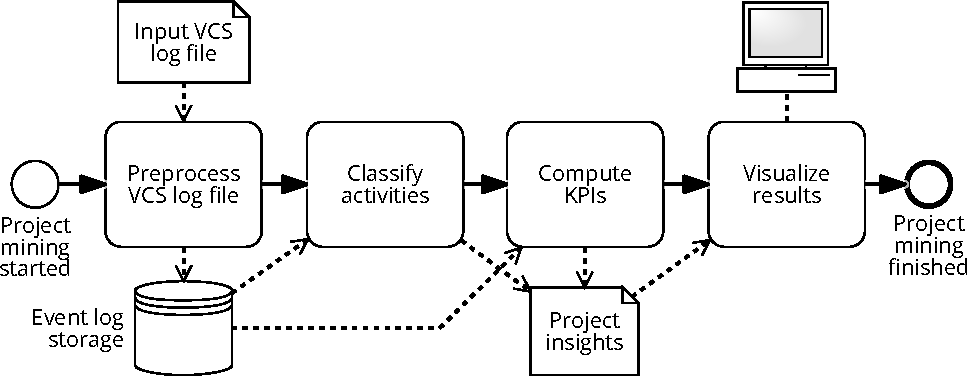
\includegraphics[width=.7\textwidth]{figures/overview}
    \caption{Overview of the approach}
    \label{fig:approach-overview}
\end{figure}


% \subsection{Implementation}

% This section presents the implementation of our technique to extract the type of work and several KPIs from a \gls{vcs} log.

\paragraph{Preprocess VCS log file.}

The input of this phase is a log in the unified diff format, which is supported
by the major \glspl{vcs}, such as Git and Subversion. The information retrieved by the \gls{vcs} is configurable by the user. More specifically, it is possible to obtain the basic information shown in \Cref{lst:git-log} along with details on the differences among versions of the same file (i.e., which and how many lines changed from version 1 to version 2 of file X). In order to extract such information, the raw event log is parsed. We used the parser from \cite{DBLP:conf/bpm/BalaRGBMS17}. This parser generates events which are then stored into a \gls{dbms} for further processing. 

\Cref{fig:er-diagram} provides the \gls{er} model to represent the entities and relationships that are needed to capture an event. The entity \textsl{Project} models the software project at hand. By including this entity in the data model, we can gather data over multiple projects and store them in the same data store. \textsl{User} is the user who performs change operations on the files. \textsl{Commit} represents the status of the repository at a given point in time. Commits must contain a revision number, a timestamp and the user who issued them. \textsl{File} is a single file of the repository identified by its full path. \textsl{Edit} captures the change as numbers of lines added to or removed from a file. This step fulfills \textbf{RQ1}.

\begin{figure}[]
    \centering
    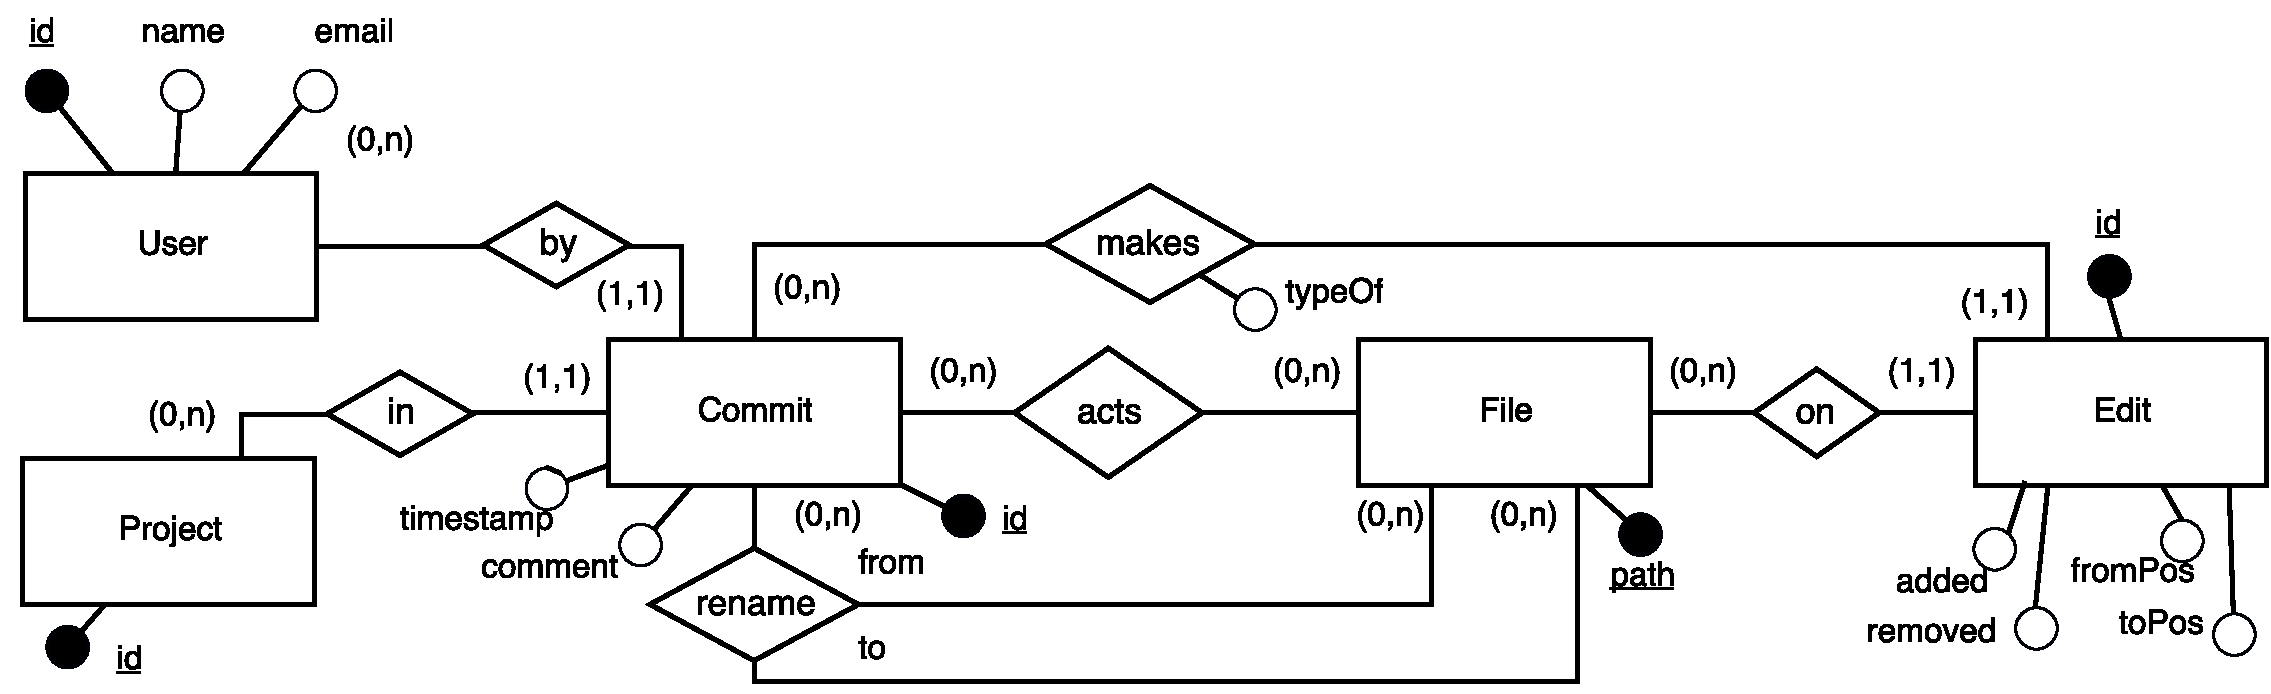
\includegraphics[width=\textwidth]{figures/CommitLogER}
    \caption{ER diagram capturing the entities and relationships of a software repository}
    \label{fig:er-diagram}
\end{figure}


\paragraph{Classify activities.}


Having the data stored in a \gls{dbms}, enables us to run several analyzes already at this level by simply issuing SQL queries. For example, we can obtain all changes that happened to single files during their lifetime. For the scope of this work, we collect all the file paths, all the changes that happened to files, the amount of change in terms of \gls{loc}, the type of change (e.g., addition, modification, deletion), the commit identifier, and the user who did the change. 
Next, we automatically categorize the type of change. For this, we apply regular expression on path attribute using the classes provided by literature~\cite{DBLP:journals/ese/VasilescuSGM14}. 
Examples of classes are  \textsl{Documentation}, \textsl{Image}, \textsl{Testing}, \textsl{Coding}, \textsl{User interface}, etc. There are in total fourteen classes. When a type of change does not belong to any class, it is put under the category \textsl{Unknown}.

% Please add the following required packages to your document preamble:
% \usepackage{booktabs}
% \usepackage{graphicx}
\begin{table}[!htbp]
\centering
\caption{Set of activities that are discovered and main regular expressions}
\label{tab:regex}
\resizebox{\textwidth}{!}{%
% \scriptsize
\begin{tabular}{@{}p{2.2cm}p{2.1cm}p{7cm}@{}}
\toprule
\multicolumn{1}{c}{\textbf{Activity}} &
  \multicolumn{1}{c}{\textbf{Abbreviation}} &
  \multicolumn{1}{c}{\textbf{Regular Expression}} \\ \midrule
  Unknown &
  unknown &
  .* \\
Documentation &
  doc &
  .*\textbackslash{}/doc(-?)book(s?)\textbackslash{}/.* .*\textbackslash{}/info .*\textbackslash{}.txt((\textbackslash{}.bak)?) .*\textbackslash{}.man .*\textbackslash{}.tex \\
Image &
  img &
  .*\textbackslash{}.jpeg .*\textbackslash{}.bmp .*\textbackslash{}.chm .*\textbackslash{}.vdx .*\textbackslash{}.gif \\
Localization &
  loc &
  .*\textbackslash{}/locale(s?)\textbackslash{}/.* .*\textbackslash{}.po($\sim$?) .*\textbackslash{}.charset($\sim$?) \\
User interface &
  ui &
  .*\textbackslash{}.ui .*\textbackslash{}.gladep(\textbackslash{}\textbackslash{}d?)((\textbackslash{}.bak)?)($\sim$?) .*\textbackslash{}.theme \\
Multimedia &
  media &
  .*\textbackslash{}.mp3 .*\textbackslash{}.mp4 .*\textbackslash{}/media(s?)\textbackslash{}/.* .*\textbackslash{}.ogg \\
Code &
  code &
  .*\textbackslash{}.jar($\sim$?) .*\textbackslash{}/src\textbackslash{}/.* .*\textbackslash{}.r((\textbackslash{}.swp)?)($\sim$?)) .*\textbackslash{}.py((\textbackslash{}.swp)?)($\sim$?) .*\textbackslash{}.php((\textbackslash{}.swp)?)(\textbackslash{}\textbackslash{}d?)($\sim$?) \\
Meta &
  meta &
  .*\textbackslash{}.svn(.*) .*\textbackslash{}.git(.*) .*\textbackslash{}.cvs(.*) \\
Configuration &
  config &
  .*\textbackslash{}.conf .*\textbackslash{}.cfg .*\textbackslash{}.project .*\textbackslash{}.ini .*\textbackslash{}.prefs \\
Build &
  build &
  .*\textbackslash{}.cmake .*\textbackslash{}/install-sh .*\textbackslash{}/build\textbackslash{}/.* .*makefile.* \\
Development documentation &
  devdoc &
  .*readme.* .*\textbackslash{}/changelog.* .*\textbackslash{}/devel(-?)doc(s?)\textbackslash{}/.* \\
Database &
  db &
  .*\textbackslash{}.sql .*\textbackslash{}.sqlite .*\textbackslash{}.mdb .*\textbackslash{}.db \\
Test &
  test &
  .*\textbackslash{}.test(s?)\textbackslash{}/.* .*\textbackslash{}/.*test\textbackslash{}..* .*/test.*\textbackslash{}..* \\
Library &
  lib &
  .*\textbackslash{}/library\textbackslash{}/.* .*\textbackslash{}/libraries\textbackslash{}/.* \\ \bottomrule
\end{tabular}%
 }
\end{table}

We have adapted the regular expressions to our case and enriched the list of rules from literature. \Cref{tab:regex} shows the activity types and the main regular expressions we use to classify files onto specific types of work. For the sake of space, the majority of the regular expressions is left out. The reader can access the full list of regular expressions on our GitHub repository whose link is provided in the following section.

\lstset{
  basicstyle={\normalsize\ttfamily}}

For the categorization we consider both the extension of the file and its path. For example, a file with the path \lstinline{/test/file.java} is labelled as \textsl{Testing} rather than \textsl{Coding}. To achieve this, we sort the matching rules in order of specificity. 
At a higher level, a commit involves multiple files. In order to fit the commit into a specific class, we rely on majority voting as follows. We iterate over the list of changes affected by the commit and sort the number of changes by their activity and the amount of change. We select the activity that is associated to the highest number of changes. With this step we fulfill \textbf{RQ2}.

\paragraph{Compute KPIs.}

According to the process already presented in \Cref{fig:approach-overview}, we compute \glspl{kpi} with the help of the \gls{dbms}. This allows for a customized set of \glspl{kpi} to be implemented. In the scope of this paper, we reproduced some of the main \glspl{kpi} form literature~\cite{DBLP:journals/ese/VasilescuSGM14}. We divide them into basic (absolute and relative) and specialization metrics. Basic metrics focus on descriptive statistics such as frequency counts of how many times each user works on a file. Specialization metrics focus on the measuring imbalance of work towards a specific file or author. Imbalance is captured by the Gini inequality index~\cite{gini1921measurement}.
We implemented the following basic project metrics: \gls{pw}, \gls{tw}, \gls{nap}, \gls{ntp}. Furthermore, we also implemented the following specialization metrics: \gls{pis}, \gls{rpis}, and \gls{rpws}. 

Let $U$ be the set of all unique users in the project, $T$ the set of all activities in the project. Files that were edited in the context of a commit can be associated to a user $u \in U$ and an activity $t \in T$ computed as described above. 
We adapted the definition of \glspl{kpi} from literature to support the extraction of information about the activity types as follows. As a first step, we redefine the two basic \glspl{kpi} that are involved in the calculation of all other \glspl{kpi}. 
%\begin{definition}[UTW]
\gls{utw} is the number of files relative to activity $t$, a user $u$ edits over the entire history of the activity.
%\end{definition}
%\begin{definition}[UTI]
\gls{uti} is 1 if a user $u$ has been involved in (i.e., has edited at least once) a file with activity $w$. It is 0 otherwise. 
%\end{definition}
Finally, using these definitions, we can present in \Cref{tab:kpis-computation} how the rest of the \glspl{kpi} is computed. With this step we fulfill \textbf{RQ3}.\\\hfill

% Please add the following required packages to your document preamble:
% \usepackage{booktabs}
% \usepackage{graphicx}
\begin{table}[]
\setlength\belowcaptionskip{-20pt}
\centering
% \scriptsize
\caption{\glspl{kpi} computation details}
\label{tab:kpis-computation}
% \resizebox{\textwidth}{!}{%
\begin{tabular}{@{}m{1.5cm}m{6cm}m{4cm}@{}}
\toprule
\textbf{KPI} & \textbf{Description}                           & \textbf{Calculation}                     \\ \midrule
\gls{pw}     & (absolute) project workload                    & $\sum_{t \in T, u \in U} \gls{utw}(t,u)$ \\
\gls{tw} (t) & workload of a specific activity  & $\sum_{u \in U} \gls{utw}(t,u) $         \\
\gls{nap}    & number of authors in the project               & $\sum_{u_j \in U} j$                     \\
\gls{ntp}    & number of activities in the project         & $\sum_{t_j \in T} j$                     \\
\gls{pis}  & specialization of user involvement the activities of the project               & $Gini_{{t_k} \in T} (\sum_{u \in U}\gls{uti}(u, t_k))$                \\
\gls{rpis} & specialization of relative user involvement over the activities of the project & $Gini_{{t_k} \in T} ( \frac{\sum_{u \in U} \gls{uti}(u, t_k)}{ \gls{nap}} ) $ \\
\gls{rpws} & specialization of relative workload across all activities in the project       & $Gini_{{t_k} \in T} ( \frac {\sum_{u \in U} \gls{utw}(u, t_k) } { \gls{tw}})$  \\ \bottomrule
\end{tabular}%
% }
\end{table}

\paragraph{Visualize results.}
The last step of our technique deals with the presentation of the results. As our prototype needs to be informative to project managers, we chose to graphically display the results of the previous two steps on a friendly user interface. The user interface takes as input the results of the classification of the activities as well as the set of the computed \glspl{kpi}. 
The main goal of the user interface is to show two fundamental aspects of the project at hand. First, it visualizes the evolution of each activity aggregated by customized periods of time (e.g., weeks, months). By doing so, our prototype helps at vizualing the general behaviour as \gls{rup} phases. This enables the project manager to compare the ideal project evolution to the actual one. Second, we display the various \glspl{kpi} in a dashboard (e.g., barchart). Further information, such as the commit identifiers, file names, amount of changes, and users who worked on the files are also made available. This allows the project manager to zoom into specific parts of the project for more detailed analyses. With this step we fulfill \textbf{RQ4}.


%%
\section{Evaluation}
\label{sec:results}

Our prototype is called ActiVCS and it is built in Java, using Java FX for the user interface. We tested its performance on a laptop with Intel\textregistered Core\texttrademark~i5-6200U CPU @ 2.30GHz x 4 processor with 8 GB of DDR4 RAM and Linux kernel 4.15.0-88-generic 64-bit version. ActiVCS takes as input a Git event log generated via the command 
\lstinline{git log --reverse --name-status > filename}. The output is presented to the user through an interactive interface. ActiVCS is publicly available and open source on GitHub (\url{https://github.com/PaulKner/ActiVCS}).
% Finally, we apply ActiVCS on thirteen real-world software projects.

\subsection{Visualization of projects}

In the following, we present the graphical interface of our prototype. 
% This work follows a design study methodology~\cite{DBLP:journals/tvcg/SedlmairMM12}. 
% It deals with a real-world problem and designs a visualization tool to support solving this problem and gather further insights for the future. In these terms, the current paper falls under the problem characterization and abstraction category. 
% In other words, our approach helps to better understand how to mine software development processes and to progress towards a fully automated software-development mining tool that is useful to project managers. In terms of suitability of the design, we argue that the 
% In these terms, the
% problem ActiVCS tackles is characterized by a \emph{rather-fuzzy task clarity} and a \emph{rather-computerized information location}. Rather-fuzzy task clarity refers to our final goal (i.e., gain insights into the current state of the project). Rather-computerized information location means that the information is mostly stored in systems. A problem with the information location in our case is that the data is scattered across several files and several versions of these files. 
% To implement ActiVCS we followed the framework of design study principles from~\cite{DBLP:journals/tvcg/LamTM18}. These principles help to bridge the analysis goals of the project manager with the tasks offered by the tool. 

% Finally, we used the nested blocks and guidelines model (NBGM)~\cite{DBLP:journals/ivs/MeyerSQM15} to design the components of our software prototype. 
% A \textsl{block} is described as the outcome of a step of the design process. Our prototype has three main blocks: the final user block, a technique block and a data block. The final user block incorporates concepts that we need to implement in order to interact with the final user. For instance, as we know that final user is a project manager, we provide him with visualization elements he is familiar with (i.e., visualization of the \gls{rup} model, \glspl{kpi} and dashboards). The technique block contains sub-blocks which implement existing techniques for classification of the type of work and computation of the \glspl{kpi}. The data block consists of sub-blocks from existing techniques to deal with raw data and the database to store these events. Another concept in the NBGM framework is that of \textsl{guideline}, which represents relationships between blocks. The blocks in our prototype are hierarchically organized. In our case, user blocks only have relationships with the technique blocks, as they need to display the results of the technique. Technique blocks have connections to all the other blocks (e.g., it is possible to analyze event log without necessarily storing them in a DB). Lastly, data blocks, besides being connected to the technique blocks,  are also connected to one anther because we may want to import/export event logs to/from the database. 

%\begin{figure}[]
%\centering
% \begin{subfigure}[b]{0.5\textwidth}
\begin{figure}
    \centering
    \includegraphics[width=\textwidth]{Project-mining-2-Mining-Type-of-Work/figures/brew0-cut}
    \caption{\gls{rup} phases mined from the \textsl{brew} project}
    \label{fig:rup-phases}
\end{figure}

\begin{figure}
    \centering
    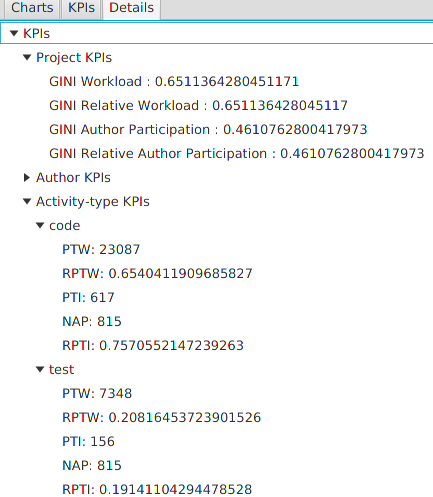
\includegraphics[width=.6\textwidth]{Project-mining-2-Mining-Type-of-Work/figures/brew3-cut}
    \caption{Detailed KPIs view of the \textsl{brew} project}
    \label{fig:brew3}
\end{figure}

\begin{figure}
    \centering
    \includegraphics[width=\textwidth]{Project-mining-2-Mining-Type-of-Work/figures/brew2-cut}
    \caption{Visualization of the effort distribution within the \textsl{brew} project}
    \label{fig:brew2}
\end{figure}

\begin{figure}
    \centering
    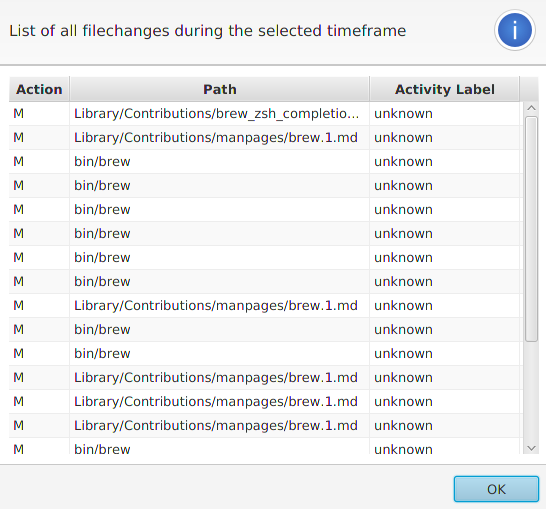
\includegraphics[width=.7\textwidth]{Project-mining-2-Mining-Type-of-Work/figures/brew1-cut}
    \caption{Details on file changes in the \textsl{brew} project}
    \label{fig:brew1}
\end{figure}

%\caption{ActiVCS applied on the real-life event log of the \textsl{brew} project}
%\label{fig:activcs-screenshots}
%\end{figure}

\Cref{fig:activcs-screenshots} shows the visualization tool in action. We extracted the \gls{vcs} log of the \textsl{brew} project from GitHub. ActiVCS has a \gls{gui} with four main frames. The main frame is depicted in \Cref{fig:rup-phases}. It allows the domain expert to execute a number of actions. These actions are the following: \begin{inparaenum}[\itshape i)] 
\item load an event log; 
\item save an event log for reuse and avoid parsing it anew;
\item get help information;
\item change granularity of the timeline by choosing to display data daily, weekly or monthly; 
\item change data series on X-axis between commit-level and file-level; and
\item four buttons to change size and type of the plots.
\end{inparaenum}
The plots shown in the frame illustrate the evolution of the identified types of work over time. Through the drop-down menu on the left pane, the user can choose between showing the classification of the activity on a commit-level or on file-level.  

It is possible to interact with each point on the plot shown in the main frame. Depending whether the X-axis is showing the information at commit-level or at file-level, a pop-up menu that summarizes the information related to that point of the plot is shown. \Cref{fig:brew1} shows this pop-up window that lists the 20 changes corresponding to a select point of the plot, in which the X-axis was set at file-level. 
\Cref{fig:brew2} presents the main \glspl{kpi} on a pane with two bar-charts and some textual information below. The barchart on the left-hand-side shows the distribution of the workload by activity. The barchart on the right-hand-side shows the number of authors who participate on each activity (i.e., have worked at least once on that activity). The text in the middle provides \glspl{kpi} about the overall project. 
\Cref{fig:brew3} shows the information presented by the fourth frame. Here it is possible to obtain details on all the \glspl{kpi} about the users (e.g. on which activities they have worked on and how much), the overall-project (e.g., the distribution of workload) and the activities (e.g., how many different activities are in the project and what is the relative work done on them). 

With this information at hand and their knowledge of the domain, the project manager can investigate, for example whether the team is \textsl{de facto} following a specific software methodology.

\subsection{Analyses of real-life open-source projects}

We use ActiVCS to analyze real-life open source projects from GitHub. 
We chose thirteen projects of different size, age, user counts, and programming languages. Selection criteria included having, 
\begin{inparaenum}[\slshape i)]
\item a representative variety in terms of programming language,
\item variety in the size,
\item at least having two similar projects,
\item highly active versus inactive, and
\item fast versus slow growing projects.
\end{inparaenum}
 

This resulted in the following projects. 
\textsl{MPAndroidChart} \textsl{(MP} is a visualization library for Android platforms. 
\textsl{Torque2D} \textsl{(Torque)} is a software engine for the development of video games. 
\textsl{Openage (openage)}	is an open source clone of the Age of Empires II engine. 
\textsl{Incubator-dubbo} \textsl{(inc)}	is a RPC (remote procedure call) framework for Java. \textsl{jekyll}	is a blog-aware written Ruby that generates websites from user content. \textsl{scrapy} is a Python based framework to extract data from 24 websites
\textsl{brew} is a software that automatically installs missing packages for MacOS and Linux operating systems. 
\textsl{Algorithms -- Java} \textsl{(Java)} is a collection of different Java algorithms. 
\textsl{Flask (flask)} is a lightweight Web Server Gateway Interface (WSGI) web application framework created in Python. 
\textsl{Tablesaw} is a framework for the transformation and visualization of data, implemented in Java.
\textsl{Okhttp (ok)} is an HTTP client for Java and Android. 
\textsl{Retrotfit (retro)}	is another HTTP client for Java and Android.
\textsl{editor.js (editor)}	is a JavaScript based editor software for the creation of documents and the transformation into JSON format.

% Please add the following required packages to your document preamble:
% \usepackage{booktabs}
\begin{table}[h]
\caption{KPIs giving insights on real-life projects.}
\label{tab:kpis-results}
% \scriptsize
\centering
\begin{tabular}{@{}crrrrrrrrrr@{}}
\toprule
\textbf{Name} &
  \multicolumn{1}{c}{\textbf{COM}} &
  \multicolumn{1}{c}{\textbf{PW}} &
  \multicolumn{1}{c}{\textbf{NAP}} &
  \multicolumn{1}{c}{\textbf{NTP}} &
  \multicolumn{1}{c}{\textbf{PWS}} &
  \multicolumn{1}{c}{\textbf{PIS}} &
  \multicolumn{1}{c}{\textbf{C}} &
  \multicolumn{1}{c}{\textbf{D}} &
  \multicolumn{1}{c}{\textbf{T}} &
  \multicolumn{1}{c}{\textbf{U}} \\ \midrule
\textit{MP}       & 2012  & 8552  & 86   & 8  & 0.8  & 0.5  & 7352  & 53    & 24   & 351  \\
\textit{Torque}   & 970   & 7978  & 46   & 9  & 0.75 & 0.34 & 5410  & 134   & 241  & 1561 \\
\textit{openage}  & 3136  & 10529 & 168  & 9  & 0.74 & 0.5  & 7697  & 596   & 366  & 1126 \\
\textit{inc}      & 3308  & 31667 & 240  & 8  & 0.69 & 0.58 & 16116 & 6     & 8232 & 164  \\
\textit{jekyll}   & 10388 & 14369 & 1028 & 9  & 0.69 & 0.6  & 4085  & 1384  & 1492 & 7001 \\
\textit{scrapy}   & 7045  & 15014 & 409  & 9  & 0.68 & 0.57 & 7995  & 612   & 2784 & 525  \\
\textit{brew}     & 18410 & 35299 & 815  & 6  & 0.65 & 0.46 & 23087 & 1276  & 7348 & 3161 \\
\textit{Java}     & 755   & 902   & 175  & 5  & 0.65 & 0.58 & 636   & 5     & 7    & 203  \\
\textit{flask}     & 3505  & 5679  & 623  & 10 & 0.65 & 0.65 & 1950  & 206   & 1027 & 481  \\
\textit{tablesaw} & 1893  & 23700 & 39   & 7  & 0.63 & 0.39 & 8779  & 11149 & 2188 & 652  \\
\textit{ok}       & 3826  & 11567 & 245  & 7  & 0.63 & 0.51 & 5837  & 225   & 3348 & 260  \\
\textit{retro}    & 1721  & 5168  & 173  & 7  & 0.6  & 0.43 & 2467  & 69    & 1039 & 103  \\
\textit{editor}   & 494   & 2337  & 27   & 7  & 0.56 & 0.24 & 927   & 314   & 0    & 814  \\ \bottomrule
\end{tabular}
\end{table}

\Cref{tab:kpis-results} shows the KPIs resulting from these projects. Columns contain the following information: number of commits (COM), \glsfirst{pw}, \glsfirst{tw}, \glsfirst{nap}, \glsfirst{ntp}, \glsfirst{pws}, \glsfirst{pis}, code (C) , documentation (D) , testing (T) and unknown (U). Entries have been sorted by the \gls{pws}.  This means that, for instance, resources of project \textsl{MP} are highly occupied. Therefore, load balancing should be considered if the managers want to improve the capacity of the team to handle new tasks in the near future. 

Finally, the types of work code (C), documentation (D), testing (T) and unknown (U) that are displayed in the table make up the most frequently identified types that were detected with ActiVCS. As expected from software development processes, the main workload in most analyzed projects were coding activities.
One exception to this observation is the jekyll project. ActiVCS has detected
7001 file changes with an unknown type within the Ruby software application. Projects like these would provide a solid basis for the identification of
additional file types. The total amount of workload that was captured across all projects is 172761. The number of file changes which could not be classified by ActiVCS and were marked as unknown is 16402. This represents 9,49\% of the total workload. Excluding the jekyll project from the analysis would reduce this margin to 5,94\%. Many of the identified projects neglect the creation of documentation.
All of the analyzed projects with a workload value for coding activities of
8000 and more also have a noticeable amount of registered testing activities.
This could refer to the fact that large software development processes
have a need for automated test activities which must be frequently updated.

%%
\subsection{Discussion}
\label{sec:discussion}

ActiVCS allows to visualize a number of \glspl{kpi} and observe patterns in the project work. It also provides a tool that can be used for checking conformance to existing software development methodologies. 
\Cref{fig:zoom} shows a screenshot of the types of work Code and Test, taken from the \textsl{ok} project, described previously. A project manager can now check that work of the type Code and Test was consistently done throughout the lifetime of the project. Moreover, it is possible to observe that Code and Test were active together most of the time, with Code starting earlier. A typical development methodology that presents such pattern is \emph{agile}. 
\begin{figure}[]
    \centering
    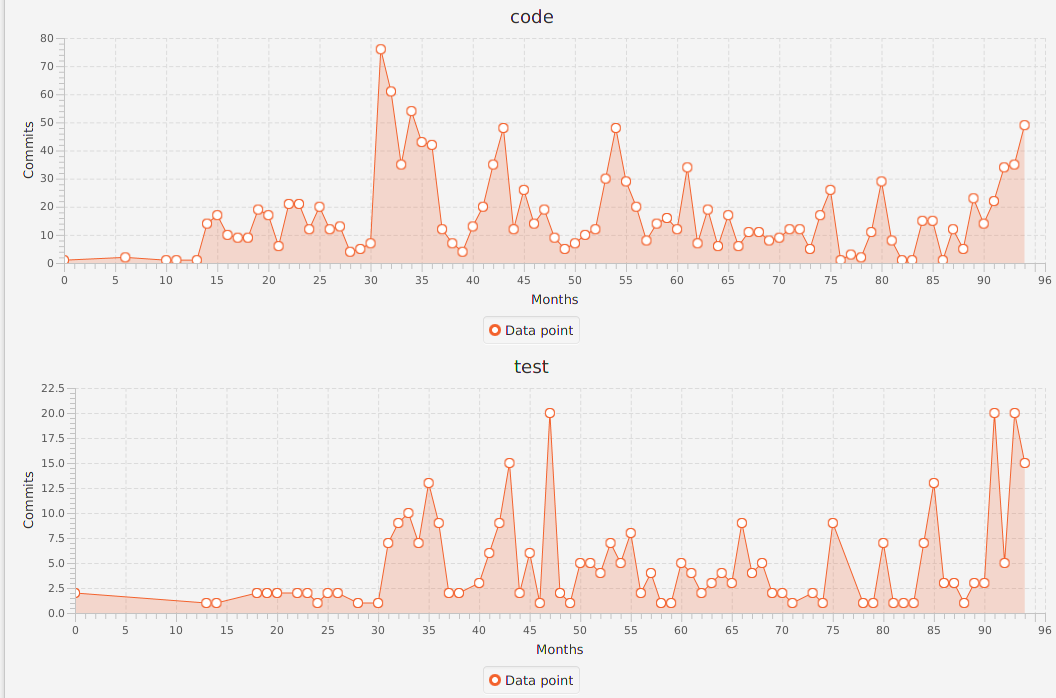
\includegraphics[width=.8\textwidth]{figures/ok-code-test}
    \caption{Zoom on the Code and Test types of work from the \textsl{ok} project}
    \label{fig:zoom}
\end{figure}


This might confirm that the \textsl{de facto} software development method corresponds with what the organization has decided. Alternatively, organization might be following a Waterfall development model. In that case, this pattern may point at a lack of control on the project. The managers can use their domain knowledge along with the provided \emph{factual} information for better decision making.

% Limitations of our technique are related to the preprocessing phase. The success of \gls{etl} procedure for obtaining the event log storage highly depends on properly formatting the \gls{vcs} log beforehand. As well, this step may be slow in case of large projects. 



%%
\section{Conclusion}
\label{sec:conclusion}

This paper provides an artifact for analyzing event logs from \gls{vcs}. Our tool is able to visualize the type of work that was executed in a software development process. Starting from fine-grained changes in the different versions of files, it allows to understand what activity was done and when. It also provides important KPIs, such as the effort distribution. These features are important for managers to understand whether the project is deviating from target goals, and in case take corrective actions.

In the future, efforts will be made to integrate the ActiVCS tool with the Gantt chart miner from~\cite{DBLP:conf/bpm/BalaCMRP}. This would offer to the project manager complementary views on the current status of the project. We plan to conduct user studies with managers in order to receive more feedback from domain experts. Finally, we have already conducted a study on selecting \glspl{kpi} for software development and we plan to incorporate them in the ActiVCS tool.

